
This Chapter returns to the Poisson equation in two dimensions.  We implement a finite element method (FEM) for an unstructured triangular mesh covering a general domain.

Our approach is to first
\begin{center}
\emph{do element-wise assembly of the residual equations,}
\end{center}
and thereby get a functioning, \pSNES-using code without even thinking about matrices as we write code.  Indeed the code can already solve certain nonlinear Poisson equations at this stage.  Only after making sure it works do we
\begin{center}
\emph{write additional code to assemble the Jacobian matrix.}
\end{center}

In this Chapter we use \PETSc for these new tasks:
\begin{itemize}
\item reading a triangular mesh from a file into \PETSc \pVecs and \pISs,
\item managing unstructured indexing of that mesh, and
\item implementing general Neumann/Dirichlet boundary conditions.
\end{itemize}

The FEM here contrasts with the structured rectangular-element ($Q^1$) FEM of Chapter \ref{chap:of} primarily in that it does not use \PETSc's \pDMDA.  We implement our own modest mesh-topology infrastructure, and, as a consequence our work-load increases substantially.  Thus we find out what we lose by not using \pDMDA, and understand better what the mesh-topology and indexing tools in \PETSc are doing.

On the other hand, this example is representative of \PETSc applications where direct contact with file formats and index sets is required.  We use the relatively-simple \texttt{triangle} program to generate ASCII files describing the mesh.  Our code uses a \PETSc \pIS type for managing the indexing of nodes and triangles.  In Chapter \ref{chap:dp} we will return to unstructured FEM methods, and there take advantage of \PETSc's \pDMPlex class for some of the unstructured mesh tasks done ``by-hand'' here.

The residual equations $\bF(\bu)=0$, as seen by the \pSNES solver, are the FEM discretization of the weak form of the PDE.  Our direct construction of these equations roughly follows the residual implementations of Chapters \ref{chap:nl} and \ref{chap:of}.  The well-known stiffness matrix $A$, and corresponding linear system $A\bx = \bb$, which form the major pieces of the standard construction in typical FEM introductions \citep{Braess2007,Elmanetal2005}, arise here as the Jacobian, and Newton step, respectively, when solving $\bF(\bu)=0$.  In our first runs, which we do before writing Jacobian-assembly user code, we allow \PETSc \pSNES to approximate this linear-system-construction through finite-differencing and (many) evaluations of $\bF$.

\section{A 2D nonlinear Poisson problem}

\begin{marginfigure}
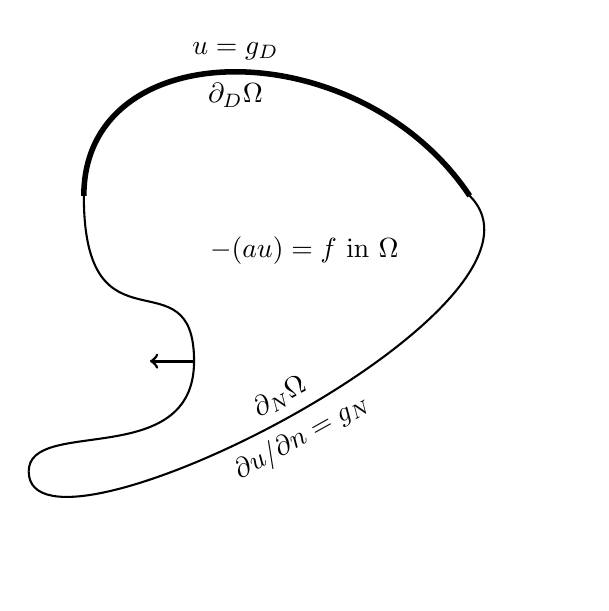
\begin{tikzpicture}[scale=0.7]
%\draw[gray,very thin] (-2,-6) grid (8,3);
\draw[line width=2pt] (0,0) .. controls (0,3) and (5,3) .. node[sloped,above] {$u=g_D$} node[sloped,below] {$\partial_D\Omega$} (7,0);
\draw[line width=0.75pt] (7,0) .. controls (9,-2) and (-1,-7) .. node[sloped,above] {$\partial_N\Omega$} node[sloped,below] {$\partial u/\partial n = g_N$} (-1,-5);
\draw[line width=0.75pt] (-1,-5) .. controls (-1,-4) and (2,-5) .. (2,-3);
\draw[line width=0.75pt] (2,-3) .. controls (2,-1) and (0,-3) .. (0,0);
\draw[->,line width=1.0pt] (2,-3) -- (1.2,-3) node[below] {$\bn$}; % normal vector
\draw (4,-1) node {$- \Div (a \grad u) = f$ in $\Omega$};
\end{tikzpicture}


\caption{Problem \eqref{eq:un:poissonstrong} on a domain.}
\label{fig:un:generalpoissondomain}
\end{marginfigure}

Let $\Omega \subset \RR^2$ be a bounded (open) region.  Suppose its boundary $\partial\Omega$ is well-behaved (polygonal or Lipschitz-continuous \citep[section 1.2]{Ciarlet2002}).  Suppose $\partial\Omega$ is decomposed into (measurable) disjoint subsets $\partial_D \Omega$ and $\partial_N \Omega$ whose union is the entire boundary $\partial \Omega$.

The Poisson problem in Chapter \ref{chap:st} is based on the equation $- \grad^2 u = f$.  We allow a more general nonlinear form here.  Let $a(x,y,u)$ and $f(x,y,u)$ be continuous functions, and assume there is $\eps>0$ so that
    $$a(x,y,u) \ge \eps > 0.$$
That is, we require \emph{uniform ellipticity} \citep{Evans2010}.  The strong form also includes boundary conditions, here nonhomogeneous Dirichlet and Neumann boundary conditions.  Thus the  nonlinear Poisson (diffusion) \emph{strong form} we solve is to find $u(x,y)$ so that
\begin{align}
- \Div \left(a(x,y,u) \grad u\right) &= f(x,y,u) \quad \text{ on } \Omega, \label{eq:un:poissonstrong} \\
u &= g_D \quad \text{ on } \partial_D \Omega, \notag \\
\frac{\partial u}{\partial n} &= g_N \quad \text{ on } \partial_N \Omega. \notag
\end{align}
By definition, $\partial u/\partial n = \bn \cdot \grad u$ where $\bn$ is the outward unit normal on $\partial \Omega$.

The data of problem \eqref{eq:un:poissonstrong}, besides the region $\Omega$ and its boundary, includes a \emph{diffusion coefficient} $a$, a \emph{source term} $f$, \emph{Dirichlet data} $g_D$, and \emph{Neumann data} $g_N$.  For the purpose of numerical solutions we will simply assume that the boundary data is continuous.  Poisson problem \eqref{poissonsquare} in Chapter \ref{chap:st} is the homogeneous Dirichlet case where $\Omega$ is the square, $a\equiv 1$, $f=f(x,y)$ is independent of the solution $u$, $\partial_D \Omega = \partial \Omega$, $\partial_N \Omega = \emptyset$, and $g_D=0$.

Problem \eqref{eq:un:poissonstrong} is not the most general (nonlinear) Poisson problem.  Specifically, one could allow more general \emph{Robin} boundary conditions $\alpha u + \beta \frac{\partial u}{\partial n} = \gamma$ where, generally, $\alpha,\beta,\gamma$ could vary along the boundary \citep{Elmanetal2005}.  One could also allow $a$ and/or $f$ to depend on the gradient of $u$, as does $a=|\grad u|^{p-2}$ in the $p$-Laplacian equation of Chapter \ref{chap:of}.

As \eqref{eq:un:poissonstrong} is stated there may be no solution where ``$\Div(a\grad u)$'' makes sense as a continuous function, even for polygonal regions and continuous data.  That is, there may be no $u\in C^2(\Omega) \cap C(\overline \Omega)$ so that $-\Div(a\grad u) = f$.  A solution exists, however, in the linear case at least, if we convert \eqref{eq:un:poissonstrong} to a \emph{weak form}.  A weak formulation arose in Chapter \ref{chap:of} as the gradient of an objective function, but the weak form here is generally not of that type.  We will derive it from the strong form in the traditional way, by multiplying by a test function and integrating.

\section{Weak form with general boundary values}

Recall $L^2(\Omega)$ is the space of square-integrable real functions on $\Omega$.  Define the following Sobolev space \citep{Evans2010}:
    $$H^1(\Omega) = \left\{u \,:\, u \in L^2(\Omega) \,\&\, \grad u \in L^2(\Omega)\right\}.$$
Definition \eqref{eq:of:sobolevdefn} of $W^{1,p}(\Omega)$ includes this space so that $H^1(\Omega) = W^{1,2}(\Omega)$.  This Chapter uses the notation with ``$H$'' standing for Hilbert.

We use two subsets of $H^1(\Omega)$: \emph{trial functions} come from $H_{g}^1(\Omega)$, which denotes the functions with value $g_D$ along $\partial_D \Omega$, and \emph{test functions} come from $H_{0}^1(\Omega)$, with value $0$ along $\partial_D \Omega$.  Note that $H_{0}^1(\Omega)$ is a linear subspace of $H^1(\Omega)$ while generally $H_{g}^1(\Omega)$ is not.

Now choose any $v\in H_{0}^1(\Omega)$, multiply the first equation in \eqref{eq:un:poissonstrong} by $v$, and integrate by parts:
\begin{equation*}
\int_\Omega a(u) \grad u \cdot \grad v - \int_{\partial\Omega} \frac{\partial u}{\partial n} v = \int_\Omega f(u) v.
\end{equation*}
(In writing such integrals we generally show dependence on the solution $u$ but suppress it for $x,y$ so that $a(x,y,u)=a(u)$, and similarly for $f$.)  Next we use the boundary information, namely that $v=0$ on $\partial_D\Omega$ and $\frac{\partial u}{\partial n}=g_N$ on $\partial_N\Omega$:
\begin{equation}
\int_\Omega a(u) \grad u \cdot \grad v = \int_\Omega f(u) v + \int_{\partial_N\Omega} g_N v\quad \text{ for any } v\in H_{0}^1(\Omega). \label{eq:un:poissonweak}
\end{equation}
Equation \eqref{eq:un:poissonweak} is the \emph{weak formulation} of \eqref{eq:un:poissonstrong}, and any $u \in H_{g}^1(\Omega)$ satisfying it is a \emph{weak solution}.  Observe that the Dirichlet boundary conditions $g_D$ are incorporated into defining $H_{g}^1(\Omega)$ while the Neumann boundary data $g_N$ appears in the weak form \eqref{eq:un:poissonweak}.

Summarizing the ``rules'' for passing between the strong \eqref{eq:un:poissonstrong} and weak \eqref{eq:un:poissonweak} formulations might clarify the situation:\begin{itemize}
\item A well-behaved function $u \in C^2(\Omega) \cap C(\overline \Omega)$ which satisfies the strong form also solves the weak form.  (The derivation above shows this.)
\item If $u \in H_{g}^1(\Omega)$ solves the weak form then we accept it, by definition, as a solution.   If it is also well-behaved (i.e.~$u \in C^2(\Omega) \cap C(\overline \Omega)$) then we may reverse the derivation to show it solves the strong form.  (Not shown, but see \citet{Evans2010}.)
\end{itemize}

Consider the linear case where functions $a$ and $f$ are independent of $u$.  If $\partial_D \Omega$ has positive measure then a solution to weak formulation \eqref{eq:un:poissonweak} exists and is unique (\emph{well-posedness}; \citep{Ciarlet2002,Evans2010}).  There exist conditions on the domain (e.g.~convex polygon) and the boundary data under which one can furthermore show that $u$ solving \eqref{eq:un:poissonweak} is in $C^2(\Omega) \cap C(\overline \Omega)$ (\emph{regularity}; \citep{Evans2010}).  Such theoretical matters are mostly beyond our scope.

In nonlinear cases each particular problem must be analyzed for well-posedness.  In terms of practical computation, particular nonlinear cases covered by our method, and solvable using our code, include 2D versions of
\begin{itemize}
\item the \emph{Bratu} equation\sidenote{See Exercise \ref{chap:nl}.\ref{exer:nl:bratu} for the 1D version.} if $a\equiv 1$ and $f=\lambda e^u$, and
\item ``uniformized'' versions of the \emph{porous medium} equation \citep{Ockendonetal2003}, in which, for example, $a=u^{m-1}+\eps$ for some $m\ge 1$ and $\eps>0$.
\end{itemize}


\section{A $P^1$ finite element method}

%FIXME: can be generalized to P^2 since $\psi_i$ keeps nodal meaning? new nodes are in 1-to-1 correspondence with triangle edges, which triangle can generate?

A FEM for the Poisson problem comes from requiring the weak formulation \eqref{eq:un:poissonweak} to be true for $u$ in a finite-dimensional subspace of $H_{g}^1(\Omega)$, and for test functions $v$ ranging over a basis of a finite-dimensional subspace of $H_{0}^1(\Omega)$.\sidenote{An FEM is \emph{conforming} if these subspace claims are accurate.  Otherwise one is guilty of \emph{variational crimes} \citep{Ciarlet2002} with \emph{nonconforming elements} \citep{Braess2007}, but such nonconforming methods may be useful.}  In the \emph{Galerkin} method here, these subspaces, built upon a triangulation of $\Omega$, will be nearly the same.

To make our test function space $H_{0}^1(\Omega)$ a true subspace of $H^1(\Omega)$ we require that $\Omega$ be polygonal, with $\partial\Omega$ a closed polygon (Figure \ref{fig:un:polygon}).  Furthermore we require that segments of $\partial\Omega$ be either entirely in $\partial_D\Omega$ or entirely in $\partial_N\Omega$.

We will assume $\partial_D\Omega$ is a closed and \emph{non-empty} set.

\begin{marginfigure}
\input{tmp/blob.tikz}
\caption{A polygonal domain $\Omega$ with $\partial_D\Omega$ in bold.}
\label{fig:un:polygon}
\end{marginfigure}

By definition, a \emph{triangulation} is a finite set of non-overlapping, non-empty open triangles $\triangle_k\subset \RR^2$ which tile $\Omega$:
\begin{equation}
\Th = \left\{\triangle_k \,\Big|\, \cup_k \overline{\triangle}_k = \overline{\Omega} \, \text{ and} \,\, \Omega_k \cap \Omega_l = \emptyset \, \text{ if } k\ne l\right\}. \label{eq:un:triangulation}
\end{equation}
We index the $K$ triangles (elements) in $\Th$ by $k=0,\dots,K-1$.  The $N$ vertices (nodes) in $\Th$ are indexed by $j=0,1,\dots,N-1$, with locations
\begin{equation*}
\bx_j = (x_j,y_j).
\end{equation*}

An example triangulation $\Th$ is shown in Figure \ref{fig:un:number-mesh}.  The subscript ``$h$'' in ``$\Th$,'' traditional notation, denotes the typical or maximum size $h$ (e.g.~diameter) of the triangles.  It serves as a reminder of our desired limit $h\to 0$.  In contrast to many references--e.g.~\citet{Elmanetal2005}, which we follow in many ways---all numbering here is zero-based, suitable for a C implementation.

\begin{marginfigure}
\input{tmp/blob.1.elenum.tikz}

\medskip

\input{tmp/blob.1.nodenum.tikz}
\caption{A triangulation of the polygon in Figure \ref{fig:un:polygon}, with element (top) and node (bottom) numbering.  There are $K=15$ elements, $N=13$ nodes, and $n_D=4$ nodes in $\partial_D\Omega$.}
\label{fig:un:number-mesh}
\end{marginfigure}

We will use $P^1$ finite elements \citep{Elmanetal2005} so that our test and trial functions are continuous and linear on each $\triangle_k$.  On each triangle $\triangle_k$, such functions have three degrees of freedom.  We make think of these as the coefficients in the linear formula $a + b x + c y$, but in fact there are better local bases than $\{1,x,y\}$; see below.

For each node $j$ there is a basis (``hat'') function  $\psi_j(x,y)$ which is linear on each triangle, continuous on all of $\overline{\Omega}$, and equal to one at only one node $j$,
\begin{equation*}
\psi_j(\bx_i) = \delta_{ij}.
\end{equation*}
See Figure \ref{fig:un:hatfunction}.  (Compare Figure \ref{fig:of:q1hat}.)  Functions $\psi_j$ are in $H^1(\Omega)$ \citep{Braess2007}, with piecewise-constant partial derivatives $\partial\psi_j/\partial x$ and $\partial\psi_j/\partial y$.  The set $\{\psi_j\}_{j=0,\dots,N-1}$ is linearly-independent.

Hat functions allow us to interpolate and extend the Dirichlet data $g_D$ from its node values in $\partial_D \Omega$ to the whole of $\overline\Omega$, a useful step in our FEM implementation.  We number the $n_D$ nodes which are in the Dirichlet boundary by $\bx_{j_l} \in \partial_D\Omega$ for $l=0,\dots,n_D-1$.  (Figure \ref{fig:un:number-mesh} shows $n_D=4$ and $j_l=l$.)  Now let $\hat g_D \in C(\overline\Omega)$ be the piecewise-linear interpolant of $g_D$ which has value zero at all nodes $\bx_j$ which are not in the Dirichlet boundary $\partial_D \Omega$:
\begin{equation}
\hat g_D(x,y) = \sum_{l=0}^{n_D-1} g_D(\bx_{j_l}) \psi_{j_l}(x,y). \label{eq:un:hatgdefine}
\end{equation}

\begin{marginfigure}
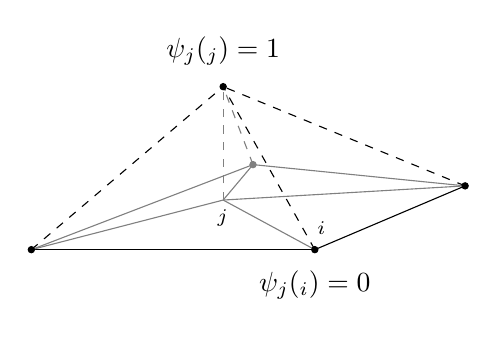
\begin{tikzpicture}[scale=0.9, z={(.707,.3)}]
    % (2,2,1) is top
    \draw[style=dashed] (0,0,0) -- (2,2,1); % to top from left
    \draw[style=dashed] (4,0,0) -- (2,2,1); %   ...  from front
    \draw[style=dashed] (4,0,3) -- (2,2,1); %   ...  from right
    \draw[color=gray, style=dashed] (0.3,0,4) -- (2,2,1); % from back
    \draw[color=gray, style=dashed] (2,0.4,1) -- (2,2,1); % from middle
    % draw base
    \draw (0,0,0) -- (4,0,0);
    \draw (4,0,0) -- (4,0,3);
    \draw[color=gray] (0,0,0) -- (0.3,0,4);
    \draw[color=gray] (0.3,0,4) -- (4,0,3);
    \draw[color=gray] (0,0,0) -- (2,0.4,1);
    \draw[color=gray] (2,0.4,1) -- (4,0,3);
    \draw[color=gray] (4,0,0) -- (2,0.4,1);
    \draw[color=gray] (2,0.4,1) -- (0.3,0,4);
    % draw \psi_j at nodes
    \filldraw (2,2,1) circle (1.25pt);
    \draw (2,2.5,1) node {$\psi_j(\bx_j)=1$};
    \draw (2,0.15,1) node {$\bx_j$};
    \filldraw (0,0,0) circle (1.25pt);
    \filldraw (4,0,0) circle (1.25pt);
    \draw (4,-0.5,0) node {$\psi_j(\bx_i)=0$};
    \draw (4.1,0.3,0) node {$\bx_i$};
    \filldraw (4,0,3) circle (1.25pt);
    \filldraw[color=gray] (0.3,0,4) circle (1.25pt);
\end{tikzpicture}


\caption{Hat functions $\psi_j$.}
\label{fig:un:hatfunction}
\end{marginfigure}

We can specify the needed finite-dimensional subspaces in terms of $\hat g_D$ and the span of certain basis functions $\psi_j$.  The \emph{test functions} are zero along $\partial_D \Omega$,
\begin{align*}
S_{0}^h &= \Span\left<\psi_j \,:\, \bx_j \notin \partial_D \Omega\right> = \Span\left<\psi_j \,:\, j \neq j_l\right>.
\end{align*}
The \emph{trial functions} have value $g_D$ along $\partial_D \Omega$,
\begin{equation}
S_{g}^h = \left\{\hat g_D + w \,:\, w \in S_{0}^h\right\}.
\end{equation}
Note that $S_{0}^h$ is a linear subspace of $H_{0}^1(\Omega)$ while $S_{g}^h$ is merely an affine subspace of $H^1(\Omega)$.  Also
\begin{equation}
\dim(S_{0}^h)=\dim(S_{g}^h)=N-n_D.
\end{equation}

The FEM itself can now be stated.  It requires \eqref{eq:un:poissonweak} to be true for $u^h\in S_{g}^h$ for all $v^h\in S_{0}^h$.  However, it suffices to consider $v^h$ from a basis of $S_{0}^h$, so we require
\begin{equation}
\int_\Omega a(u^h) \grad u^h \cdot \grad \psi_i = \int_\Omega f(u^h) \psi_i + \int_{\partial_N\Omega} g_N \psi_i \label{eq:un:weakformhat}
\end{equation}
for all $i$ such that $\bx_i \notin \partial_D \Omega$.  On the other hand we may write $u^h$ using $N-n_D$ unknown coefficients $u_j\in\RR$:
\begin{equation}
u^h(x,y) = \hat g_D(x,y) + \sum_{\bx_j \notin \partial_D \Omega} u_j\, \psi_j(x,y). \label{eq:un:uhexpand}
\end{equation}

The coefficients $u_j$ in \eqref{eq:un:uhexpand} are the unknowns.  Given the triangulation $\mathcal{T}_h$ of $\Omega$ and the data of the problem, namely the functions $a$, $f$, $g_D$, and $g_N$, the complete specification of the FEM solution $u^h$ is given by equations \eqref{eq:un:hatgdefine}, \eqref{eq:un:weakformhat}, and \eqref{eq:un:uhexpand}.

In the linear case it is common to now write system \eqref{eq:un:weakformhat} and \eqref{eq:un:uhexpand} as a linear system $A \bu = \bb$.  That is, the usual next step in an FEM is to assemble the \emph{stiffness matrix} $A$ \citep{Elmanetal2005}.  Here we will not do so until we have an initial, and verified, numerical solution.  Following the pattern established since Chapter \ref{chap:nl}, we first implement equation \eqref{eq:un:weakformhat} as a residual-evaluation function $\bF(\bu)$, from the representation of $u^h$ as a vector $\bu$, giving a nonlinear system $\bF(\bu) = 0$.  In evaluating $\bF$ we use \eqref{eq:un:uhexpand} to get point values of $u^h$ and its gradient $\grad u^h$ on the interior of triangles.  These point values allow quadrature, similar to that in Chapter \ref{chap:of}, to approximate the integrals in \eqref{eq:un:weakformhat}.  Implementing a residual in the linear case is mathematically equivalent to assembling $A$ and $\bb$, but the residual-evaluation code here is simpler because it does not require direct contact with a \pMat object at all.

In the next section we describe and the code the element-wise ``assembly,'' that is, evaluation of, the residual function $\bF$, as a \pSNES call-back.  Before that can be written we will be more specific about what \eqref{eq:un:weakformhat} says on each element, and we will read-in the triangular mesh and put it into \PETSc data structures.  These tools can be tested for correctness with a finite-differenced Jacobian (Chapter \ref{chap:nl}).  Once this is all shown to work correctly, via comparison to an exact solution, then we will re-consider matrix assembly, namely for the Jacobian derivative of $\bF$.


\section{Assembly of the residual equations}

Expression \eqref{eq:un:uhexpand} shows that $N-n_D$ real values $\{u_j\}$, for $j$ such that $\bx_j \notin \partial_D \Omega$, are needed to determine the FEM solution $u^h$.  However, it will be easier to write code if we \emph{increase} the size of the resulting nonlinear system, up to dimension $N$, by including the values of $u^h$ at nodes in the Dirichlet boundary as unknowns.  Thus we define
\begin{equation}
\bu = \{u_j\}_{j=0}^{N-1} \in \RR^N  \label{eq:un:unknowns}
\end{equation}
as the description of the FEM solution.

To enforce the boundary conditions, the components of the residual corresponding to Dirichlet boundary must be zero:
\begin{equation}
F_i(\bu) = u_i - g_D(\bx_i) \qquad \text{ if } \bx_i \in \partial_D\Omega.  \label{eq:un:dirichletresiduals}
\end{equation}

Because triangulation $\mathcal{T}_h$ satisfying \eqref{eq:un:triangulation} almost\sidenote{The set $\Omega \setminus \cup_k \triangle_k$ has measure zero.} covers $\Omega$ with non-overlapping triangles, we can write the weak form \eqref{eq:un:weakformhat} as a sum over elements.  To be specific, for each $\triangle_k \in \mathcal{T}_h$, $k=0,\dots,K-1$, let
\begin{equation}
F_i^k(\bu) = \int_{\triangle_k} a(u^h) \grad u^h \cdot \grad \psi_i - f(u^h) \psi_i.  \label{eq:un:elementweakform}
\end{equation}
Suppose $n_N$ is the number of edges which are in the Neumann boundary.  We call these edges (Neumann) \emph{segments} for distinctive language.  For each segment $s_\nu$, $\nu=0,\dots,n_N-1$, let
\begin{equation}
\varphi_i^\nu = \int_{s_\nu} g_N \psi_i.  \label{eq:un:segmentweakform}
\end{equation}
(These values do not depend on the solution $u^h$.)  Then residual equation \eqref{eq:un:weakformhat} is
\begin{equation}
F_i(\bu) = \sum_{k=0}^{K-1} F_i^k(\bu) + \sum_{\nu=0}^{n_N-1} \varphi_i^\nu = 0  \qquad \text{ if } \bx_i \notin \partial_D\Omega. \label{eq:un:elementwisesum}
\end{equation}
Together, equations \eqref{eq:un:dirichletresiduals} and \eqref{eq:un:elementwisesum} form the (generally) nonlinear system, of dimension $N$, which we hand to a \pSNES solver:
\begin{equation}
\bF(\bu)=0. \label{eq:un:fullsystem}
\end{equation}

Observe that $n_D$ is the number of \emph{nodes} in the Dirichlet boundary, whereas $n_N$ is the number of \emph{segments} (edges) in the Neumann boundary.  The former correspond to degrees of freedom, while the latter are domains of integration.  Managing the mesh correctly requires making this distinction.

Because the support of the hat function $\psi_i$ only overlaps with a few triangles $\triangle_k$, for each $i$ only a few values $F_i^k(\bu)$ and $\varphi_i^\nu$ are nonzero.  Also, only a few nodal values $\bu=\{u_j\}$ enter into $F_i^k(\bu)$, namely those values $u_j$ such that the support of $\psi_j$ overlaps with $\triangle_k$.  These facts make \eqref{eq:un:fullsystem} a \emph{sparse} nonlinear system.  The Jacobian $J_\bF(\bu)$ is, therefore, a sparse matrix.

We will compute the element integrals \eqref{eq:un:elementweakform} by referring $\triangle_k$ to a reference triangle $\triangle_\ast$ with vertices $(0,0),\,(1,0),\,(0,1)$, as shown in Figure \ref{fig:isoparametric}.  In Chapter \ref{chap:of} we did the same thing for quadrilaterals, so here we can be relatively brief.

If $\triangle_k$ has vertices $(x_0,y_0),\,(x_1,y_1),\,(x_2,y_2)$ then the linear map from $\triangle_\ast$ to $\triangle_k$ is
\begin{align}
x(\xi,\eta) &= x_0 + (x_1-x_0) \xi + (x_2-x_0) \eta, \label{eq:un:trianglemap} \\
y(\xi,\eta) &= y_0 + (y_1-y_0) \xi + (y_2-y_0) \eta. \notag
\end{align}
The Jacobian determinant $\det J_k$ of map \eqref{eq:un:trianglemap}, needed for change-of-variables to integrate over the reference element, is a constant on each element.  Its magnitude is the ratio of the area of $\triangle_k$ to the area of the reference element $\triangle_\ast$.  See Exercise \ref{chap:un}.\ref{exer:un:gradientdetails}.

\begin{marginfigure}
\begin{tikzpicture}[scale=1.1,
    decoration={
      markings,
      mark=at position 1 with {\arrow[scale=1.8,gray]{latex}};
    }]
% left x,y axes
    \draw[->, gray, very thin] (1.5,0) -- (4.0,0);
    \draw[->, gray, very thin] (2,-0.5) -- (2,2.4);
    \draw (4.1,-0.1) node {$x$};
    \draw (1.9,2.4) node {$y$};
    \filldraw (1.7,1) circle (1.25pt);    % (x_0,y_0)
    \filldraw (3.5,-0.3) circle (1.25pt); % (x_1,y_1)
    \filldraw (3.0,2.0) circle (1.25pt);  % (x_2,y_2)
    \draw (1.4,1.3) node {$(x_0,y_0)$};
    \draw (3.5,-0.6) node {$(x_1,y_1)$};
    \draw (3.0,2.3) node {$(x_2,y_2)$};
    \draw[line width=1pt] (1.7,1) -- (3.5,-0.3) -- (3.0,2.0) -- cycle;
    \draw (2.7,1.0) node {$\triangle_k$};
% right xi,eta axes
    \draw[->, gray, very thin] (4.6,0) -- (6.6,0);
    \draw[->, gray, very thin] (5,-0.4) -- (5,2.0);
    \draw (6.7,-0.1) node {$\xi$};
    \draw (4.9,2.05) node {$\eta$};
    \filldraw (5,0) circle (1.25pt);  % (0,0)
    \filldraw (6,0) circle (1.25pt);  % (1,0)
    \filldraw (5,1) circle (1.25pt);  % (0,1)
    \draw (5.2,-0.3) node {$0$};
    \draw (6.2,0.2) node {$1$};
    \draw (5.2,1.1) node {$2$};
    \draw[line width=1pt] (5,0) -- (6,0) -- (5,1) -- cycle;
    \draw (5.3,0.3) node {$\triangle_\ast$};
% arrows connecting nodes
    \draw[gray, postaction={decorate}] (5,0) -- (1.7,1.03);
    \draw[gray, postaction={decorate}] (6,0) -- (3.5,-0.3);
    \draw[gray, postaction={decorate}] (5,1) -- (3.0,2.0);
\end{tikzpicture}


\caption{Mapping of a triangle $\triangle_k$ from the reference triangle $\triangle_\ast$.}
\label{fig:isoparametric}
\end{marginfigure}

On $\triangle_\ast$ any linear function is a linear combination of three local (nodal) basis functions:
\begin{equation}
\chi_0(\xi,\eta) = 1-\xi-\eta, \qquad \chi_1(\xi,\eta) = \xi, \qquad \chi_2(\xi,\eta) = \eta. \label{eq:un:chiformulas}
\end{equation}
If $\bx_i\in\overline{\triangle_k}$ then hat function $\psi_i$ satisfies
\begin{equation}
\psi_i(x(\xi,\eta),y(\xi,\eta)) = \chi_\ell(\xi,\eta) \label{eq:un:psichimap}
\end{equation}
for all $(\xi,\eta)\in\triangle_\ast$, where vertex $\ell$ of $\triangle_\ast$ maps to $\bx_i$.

Recalling both the change-of-variables formula for integrals and the chain rule, we can write
\begin{equation}
F_i^k(\bu) = |\det J_k| \int_{\triangle_\ast} H_\ell^k(\bu,\xi,\eta)\,d\xi\,d\eta \label{eq:un:elementintegralreference}
\end{equation}
where the integrand is
\begin{equation}
H_\ell^k(\bu,\xi,\eta) = \left[a(u^h) \grad u^h \cdot \grad \psi_i - f(u^h) \psi_i\right]_{\triangle_\ast}.  \label{eq:un:elementintegrand}
\end{equation}
Here the vertex $\ell \in \{0,1,2\}$ of $\triangle_\ast$ corresponds to the node $\bx_i$.  Note that ``$\grad$'' in \eqref{eq:un:elementintegrand} refers to derivatives in variables $x,y$.  Exercises \ref{chap:un}.\ref{exer:un:gradientdetails} and \ref{chap:un}.\ref{exer:un:elementintegranddetails} addresses the details implicit in \eqref{eq:un:elementintegralreference} and \eqref{eq:un:elementintegrand}.

As in Chapter \ref{chap:of}, the integrals \eqref{eq:un:elementintegralreference} will be approximated using quadrature.  Generally, if there are $Q$ quadrature points $(\xi_q,\eta_q) \in \triangle_\ast$ with weights $w_q$ then
\begin{equation}
F_i^k(\bu) \approx |\det J_k| \sum_{q=0}^{Q-1} w_q H_\ell^k(\bu,\xi_q,\eta_q). \label{eq:un:elementquadraturereference}
\end{equation}

Unlike in Chapter \ref{chap:of}, however, the elements are not rectangular.  Quadrature rules based on products of one-dimensional integrals can be built \citep{KarniadakisSherwin2013}, but here we use rules constructed for the reference triangle $\triangle_\ast$.  Some cases which are exact for polynomials of degrees $1,2,3$ appear in Table \ref{tab:un:quadrature}.  These are symmetrical Gaussian rules \citep{Dunavant1985} with $Q=1,3,4$ points, respectively (Exercise \ref{chap:un}.\ref{exer:un:checkquadrature}).  Note that the sum of the weights is $1/2$ because the area of $\triangle_\ast$ is $1/2$.

\begin{table}[h]
\vspace{0.1in}

\begin{tabular}{lccc}
degree & $Q$ & weights $w_q$ & nodes $(\xi_q,\eta_q)$ \\ \hline
$1$ & $1$ & $1/2$ & $(1/3,1/3)$ \\ \hline
$2$ & $3$ & \begin{tabular}{c}
            $1/6$ \\
            $1/6$ \\
            $1/6$
            \end{tabular} & \begin{tabular}{c}
            $(1/6,1/6)$ \\
            $(2/3,1/6)$ \\
            $(1/6,2/3)$
            \end{tabular} \\ \hline
$3$ & $4$ & \begin{tabular}{c}
            $-27/96$ \\
            $25/96$ \\
            $25/96$ \\
            $25/96$
            \end{tabular} & \begin{tabular}{c}
            $(1/3,1/3)$ \\
            $(1/5,1/5)$ \\
            $(3/5,1/5)$ \\
            $(1/5,3/5)$
            \end{tabular}
\end{tabular}

\vspace{0.1in}
\caption{Symmetric quadrature rules, on the reference triangle $\triangle_\ast$, used to compute \eqref{eq:un:elementquadraturereference}.} \label{tab:un:quadrature}
\end{table}


\section{Triangular meshes from \Triangle}

\PETSc itself does not include tools for triangulating regions of the plane.  We use the widely-available \Triangle\sidenote{See \href{http://www.cs.cmu.edu/~quake/triangle.html}{www.cs.cmu.edu/$\sim$quake/ triangle.html} for documentation and source code.} software \citep{Shewchuk1996} for this task.  \Triangle is limited to 2D, and it only writes ASCII files, but it has straightforward details.

As input to describe a polygonal region $\Omega$, \Triangle uses an ASCII file with extension \texttt{.poly}.  This input also indicates Dirichlet and Neumann portions of the boundary $\partial \Omega$.  For example, the polygon shown in Figure \ref{fig:un:polygon} was created from the hand-built input file \texttt{blob.poly} shown in Code \ref{code:blobpoly}.  Note that \Triangle takes and generates files with 1-based indexing.

\inputfromline{../c/\CODELOC/meshes/blob.poly}{\CODELOC blob.poly}{A description of the boundary polygon in Figure \ref{fig:un:polygon}, suitable for reading by \Triangle.}{8}{code:blobpoly}

The triangulation shown in Figure \ref{fig:un:number-mesh} came from a single command which asks \Triangle to generate a triangulation, for the \texttt{blob.poly} polygon, which has a polygon output file (option \texttt{-p}), relatively-uniform triangles (option \texttt{-q} for ``quality-checked'' \citep{Shewchuk1996}), and triangles with maximum area of $4.0$ (option \texttt{-a4.0}):
\begin{cline}
$ triangle -pqa4.0 blob
\end{cline}
%$
This command generates three ASCII files, \texttt{blob.1.poly}, \texttt{blob.1.node}, and  \texttt{blob.1.ele}.  These files define the polygonal boundary, node locations, and elements in the triangulation, respectively.

\Triangle includes a minimal visualization tool.  The command
\begin{cline}
$ showme blob
\end{cline}
%$
displays the boundary polygon (from \texttt{blob.poly} or \texttt{blob.1.poly}) and the triangulation itself (\texttt{blob.1.node} and \texttt{blob.1.ele}).


\section{From ASCII files to \PETSc \pIS and \pVec}

FIXME: Will put \texttt{.node} into \pVec, \texttt{.ele} into \pIS, Dirichlet/Neumann marker into \pIS.  Will read ASCII into Python (not C) and write out \pVec, \pIS with \texttt{PetscBinaryIO.py}.  Then \texttt{unfem.c} will read \pVec, \pIS with \texttt{VecLoad(),ISLoad()}

FIXME: YES WE DO THIS IN Python NOW.  The ASCII files produced by \Triangle are not in a good format for large meshes, but we will accept this for portability and readability.  We will, however, demonstrate how files are read in parallel, based on first doing a mundane and un-scalable task in \PETSc, namely reading the ASCII \Triangle files serially, in a Python program, and writing out a binary file in \PETSc format.  Of course we will focus on the scalability of the FEM solution process, once the mesh is loaded.

FIXME THIS IS STILL A VALID POINT  In this part there is an important detail about triangulations, which affects the data structure for elements.  Namely, we cannot tell if an edge of an element is in the boundary just by whether both endpoints are in the boundary.  For example, edge from node 5 (on the Dirichlet boundary) to node 7 (on the Neumann boundary) in Figure \ref{fig:un:number-mesh} is not in the boundary.  Thus we need to have list of flags for the boundary segments themselves.


\section{Assembling an approximate Jacobian}

FIXME EXPLAIN PICARD $\bF(\bu)=0$ to $A(\bu) \bu - \bb(\bu)=0$ to $A(\bu^k) \bu^{k+1} - \bb(\bu^k)=0$ to $A(\bu^k) (\bu^{k+1}-\bu^k) - \bb(\bu^k)= - A(\bu^k) \bu^k$ to $A(\bu^k) \bs = -\bF(\bu^k)$

FIXME Furthermore we do it in parallel.  Recall that \texttt{c3convert.c} above creates a distributed \pVec called \texttt{E}, which is an array of elements of type \texttt{elementtype}, and \texttt{readmesh.c} reads it.

FIXME For the element-by-element assembly procedure we first define the integral over one triangle $\triangle_k$,
\begin{equation}
\text{\texttt{a(k,i,j)}} = \int_{\triangle_k} a(u^h) \grad \psi_i \cdot \grad \psi_. \label{aelementintegral}
\end{equation}
so that
    $$\tilde a_{ij} = \sum_k \phantom{.}\text{\texttt{a(k,i,j)}}.$$
Likewise we will compute
\begin{equation}
\text{\texttt{b(k,i)}} = \int_{\triangle_k} f \psi_i + \int_{\overline{\triangle}_k \cap \partial_N\Omega} g_N \psi_i, \label{belementintegral}
\end{equation}
so that $\tilde b_i = \sum_{k} \;\text{\texttt{b(k,i)}}$.


FIXME IS NOW THE JACOBIAN This linear system
\begin{equation}
A \bu = \bb, \label{poissonmatrix}
\end{equation}
has $A\in\RR^{N\times N}$ and $\bu,\bb\in\RR^N$, where $N$ is the number of nodes.  \pMat and \pVec objects store the problem

FIXME $A$ is \emph{symmetric}, $a_{ij}=a_{ji}$ and \emph{sparse}

FIXME For the right side define the entries
\begin{equation}
    b_i = \int_\Omega f \psi_i + \int_{\partial_N\Omega} \gamma \psi_i - \sum_{l=0,\dots,L} g(\bx_{j_l})  \int_\Omega \grad \psi_{j_l} \cdot \grad \psi_i  \label{bentryfem}
\end{equation}
if $\bx_i \notin \partial_D \Omega$, while if $\bx_i \in \partial_D \Omega$ then
    $$b_i = g(\bx_{i}).$$


%\section{Preallocate a \pMat}
%FIXME: figure showing parallel partition of elements
%\cinputpart{testprealloc.c}{Read mesh \pVecs from file.  Get row ownership range.}{I}{//STARTLOAD}{//ENDLOAD}{code:testpreallocpartone}
%\cinputpart{testprealloc.c}{Set up \pMat $A$ and actually preallocate it.  Fill it with junk entries so the pattern can be visualized.}{II}{//ENDLOAD}{//ENDTEST}{code:testpreallocparttwo}


\begin{comment}
   The "trick" is that first partition the element across processes, then partition the vertices (nodal values) subservient to the partitioning of the elements and then you "renumber" the elements and vertices so that the elements on the first process are numbered first, followed by the elements on the second process etc and similarly the vertices on the first process are numbered before the vertices on the second processes etc.

  Now each process just needs to loop over its elements compute the element stiffness/load and call MatSetValues/VecSetValues() the the "new" numbering of the vertices.  The "old" numbering that was on the disk is simply not used in communicating with PETSc, you only use the new PETSc numbering.

   Barry

> On Apr 26, 2016, at 1:03 PM, Jie Cheng <chengj5@rpi.edu> wrote:
>
> Hello everyone
>
> I have a finite element code to solve nonlinear solid mechanics (using Newton-Raphson iteration) implemented with PETSc. The code is serial, organized as following:
>
> 1) Read the connectivity of the unstructured mesh, coordinates of nodes from individual txt files.
> 1.1) Connectivity file contains [# of elements] rows, and each row lists the global number of nodes on that element. Take 3d hexahedral elements for instance:
>       223 224 298 297 1 2 76 75
>       224 225 299 298 2 3 77 76
>       ? ?
> 1.2) Coordinates file contains [# of nodes] rows, and each row lists the coordinates of a node, for example:
>       0                   0.0011                      3.9e-5
>       2.3677e-5     0.001.9975                3.9e-5
>       ? ?
>
> 2) Create the global stiffness A matrix with MatCreateSeqAIJ since the dimensions and nonzero pattern are known from the connectivity.
> 3) Loop over the element to compute the element stiffness matrix and right hand side. Then assemble the global stiffness matrix and right hand side.
> 4) Solve the linear equation with KSPsolve for the displacement increment, then go back to Step 3.
>
> The code works fine in serial, now I?m trying to parallelize it. To partition the mesh, I can use partdmesh from METIS, or let PETSc calls it. Either way I will find a way to assign different elements and nodes to different ranks. My question is: since PETSc does not allow us to control the memory distribution of the parallel matrix/vector, how do I make sure the rank happens to have all/most memory it needs for the specific elements? For example, rank 0 is in charged of element n, and needs to insert values to A[ i ][ j ], how do I make sure the i-th row is assigned to rank 0?
>
> This question is fundamental for people work with finite element methods. I checked the tutorial codes but did not find an example to follow. Section 3.5 of the manual talks about partition, but it does not say anything about linking the partition with the memory distribution. Could anyone give me some instructions on this issue? Thank you in advance!
>
> Best
> Jie Cheng
\end{comment}




\section{Exercises}

\renewcommand{\labelenumi}{\arabic{chapter}.\arabic{enumi}\quad}
\renewcommand{\labelenumii}{(\alph{enumii})}
\begin{enumerate}
\item  \label{exer:un:gradientdetails}  For the map \eqref{eq:un:trianglemap} from $\triangle_\ast$ to $\triangle_k$, let
    $$J_k = \frac{\partial (x,y)}{\partial (\xi,\eta)} = \begin{pmatrix}
    x_1 - x_0 & x_2 - x_0 \\
    y_1 - y_0 & y_2 - y_0 \end{pmatrix}
    = \begin{pmatrix}
    \Delta x_1 & \Delta x_2 \\
    \Delta y_1 & \Delta y_2
    \end{pmatrix}$$
be the Jacobian.  Use the chain rule and \eqref{eq:un:psichimap} to show that
\begin{equation}
\grad_{x,y} \psi_i = \frac{1}{\det J_k} \left<\Delta y_2 \frac{\partial \chi_\ell}{\partial \xi} - \Delta y_1 \frac{\partial \chi_\ell}{\partial \eta}, - \Delta x_2 \frac{\partial \chi_\ell}{\partial \xi} + \Delta x_1 \frac{\partial \chi_\ell}{\partial \eta}\right>. \label{eq:un:gradpsionref}
\end{equation}
Here indices $i$ and $\ell$ have the same relationship as in \eqref{eq:un:psichimap}.  Comparing formula \eqref{eq:of:gradpsionref} for the structured case, what is the underlying reason why \eqref{eq:un:gradpsionref} is a bit more complicated?  % underlying reason is that affine map here includes rotations, while in Chapter \ref{chap:of} it was just translation and axes scaling
\item  \label{exer:un:elementintegranddetails}  Formula \eqref{eq:un:elementintegrand} might require some interpretation before the implementation becomes clear.  Confirm that, with only mild abuses of notation, formulas \eqref{eq:un:trianglemap} and \eqref{eq:un:psichimap} lead to the valid expansions
\begin{align*}
a(u^h) &= a(u^h,\xi,\eta) = a(u^h,x(\xi,\eta),y(\xi,\eta)), \\
f(u^h) &= f(u^h,\xi,\eta) = f(u^h,x(\xi,\eta),y(\xi,\eta)), \\
\psi_i &= \chi_{\ell}(\xi,\eta), \\
u^h &= \sum_{j=0}^{N-1} \left\{\begin{matrix} g_D(\bx_j) \\ u_j \end{matrix}\right\} \chi_{\ell'}(\xi,\eta), \\
\grad u^h &= \grad_{x,y} u^h = \sum_{j=0}^{N-1} \left\{\begin{matrix} g_D(\bx_j) \\ u_j \end{matrix}\right\} \grad_{x,y} \psi_j.
\end{align*}
For the third formula, node $\bx_i$ corresponds to vertex $\ell$ on $\triangle_\ast$.  In the fourth and fifth formulas, node $\bx_j$ corresponds to vertex $\ell'$ on $\triangle_\ast$, and the two cases for the coefficient are when $\bx_j \in \partial_D \Omega$ and $\bx_j \notin \partial_D \Omega$, respectively.  Note that \eqref{eq:un:gradpsionref} allows us to expand $\grad_{x,y} \psi_j$ in the fifth formula.  Taken together, these expansions make \eqref{eq:un:elementintegrand} meaningful and implementable.
\item  \label{exer:un:checkquadrature}  The degree of accuracy $n=1,2,3$ of the quadrature rules in Table \ref{tab:un:quadrature} can be checked by comparing the exact integral
\begin{equation}
\iint_{\triangle_\ast} \xi^i \eta^j\,d\xi d\eta = \frac{i!\,j!}{(i+j+2)!}, \label{eq:un:checkquadrature}
\end{equation}
for all cases with $0\le i+j\le n$, against the quadrature result.  Also one should show an inexact quadrature result for some case with $i+j=n+1$.  Write a small program, in the language of your choice, which does these things.
\end{enumerate}

